\documentclass[tikz, border = 10pt]{standalone}

\usepackage{newpxtext,newpxmath}   % /upbeta
%\usepackage{fouriernc}            % /otherbeta
\usepackage{amsmath}
\renewcommand{\familydefault}{\sfdefault}
\usepackage{mathastext}

\usetikzlibrary{positioning, quotes, calc, math, arrows.meta, bending, shapes, backgrounds}

\tikzset{
every edge quotes/.style = {fill = white},
every node/.style = {scale = 1.1},
manifest/.style = {rectangle, draw, thin, inner sep = 3pt, minimum width = 1cm,
   minimum height = .85cm, align = center},
latent/.style = {ellipse, draw, thin, inner sep = 3pt, minimum width = 1cm,
   minimum height = .85cm},
residual1/.style = {circle, draw, thin, minimum size = 5mm, inner sep = 1pt},
residual2/.style = {rectangle, minimum width = 0.5pt, minimum height = 1.5mm,
   inner sep = 0pt, outer sep = 0mm},
regression/.style = {-{Stealth[length = 1.5mm]}, thin, shorten > = 1pt, 
   inner sep = 1.5pt, outer sep = 0mm},
covariance/.style={{Stealth[length = 1.5mm]}-{Stealth[length = 1.5mm]}, thin,
   shorten > = 1pt, shorten < = 1pt, inner sep = 1.5pt},
variance/.style={{Stealth[length = 1mm]}-{Stealth[length = 1mm]}, thin,
   shorten > = 1pt, shorten < = 1pt, inner sep = 1pt},
interaction/.style = {-{Stealth[sep = 1pt, length = 1.5mm] . Circle[length = 4pt]},
   thin, shorten > = -2pt},
constant/.style = {draw, thin, inner sep = 1pt, regular polygon,
   regular polygon sides = 3, minimum size = 5mm},
group/.style = {rectangle, inner sep = 2pt, minimum width = 15mm, minimum height = 5mm, 
   align = center}
}

\begin{document}
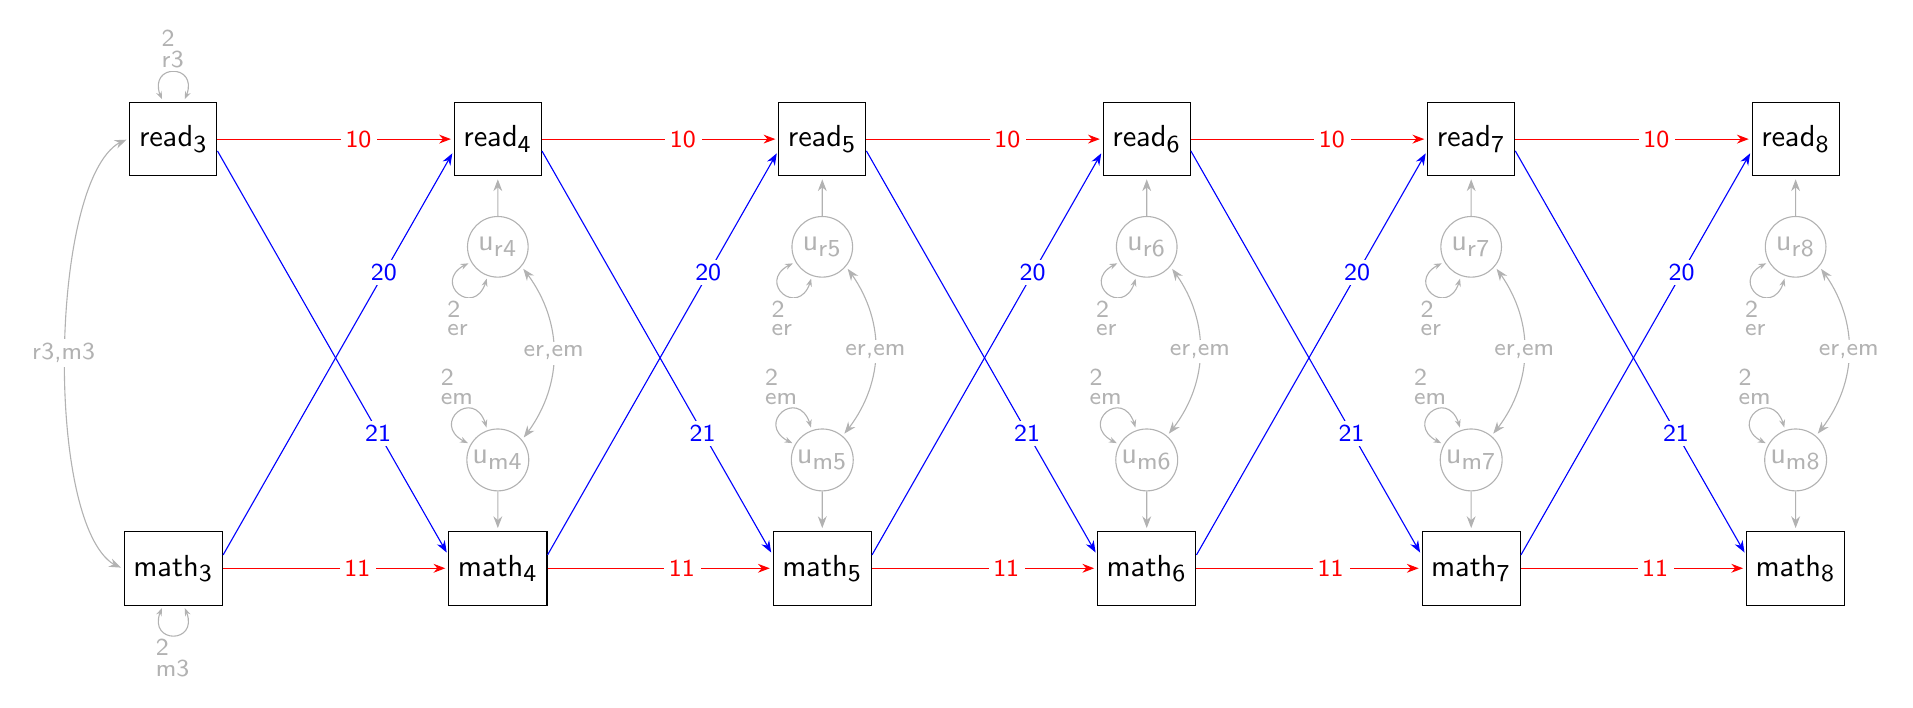
\begin{tikzpicture}

%% Manifest
\node [manifest] (x1) {read$_3$};
\node [manifest] (x2) [right = 3cm of x1] {read$_4$};
\node [manifest] (x3) [right = 3cm of x2] {read$_5$};
\node [manifest] (x4) [right = 3cm of x3] {read$_6$};
\node [manifest] (x5) [right = 3cm of x4] {read$_7$};
\node [manifest] (x6) [right = 3cm of x5] {read$_8$};

\node [manifest] (y1) [below = 4.5cm of x1] {math$_3$};
\node [manifest] (y2) [below = 4.5cm of x2] {math$_4$};
\node [manifest] (y3) [below = 4.5cm of x3] {math$_5$};
\node [manifest] (y4) [below = 4.5cm of x4] {math$_6$};
\node [manifest] (y5) [below = 4.5cm of x5] {math$_7$};
\node [manifest] (y6) [below = 4.5cm of x6] {math$_8$};

%% Regressions - Stability
\path [regression, red] (x1) edge ["$\upbeta_{10}$", pos = 0.6] (x2); 
\path [regression, red] (x2) edge ["$\upbeta_{10}$", pos = 0.6] (x3); 
\path [regression, red] (x3) edge ["$\upbeta_{10}$", pos = 0.6] (x4); 
\path [regression, red] (x4) edge ["$\upbeta_{10}$", pos = 0.6] (x5); 
\path [regression, red] (x5) edge ["$\upbeta_{10}$", pos = 0.6] (x6); 

\path [regression, red] (y1) edge ["$\upbeta_{11}$", pos = 0.6] (y2); 
\path [regression, red] (y2) edge ["$\upbeta_{11}$", pos = 0.6] (y3); 
\path [regression, red] (y3) edge ["$\upbeta_{11}$", pos = 0.6] (y4); 
\path [regression, red] (y4) edge ["$\upbeta_{11}$", pos = 0.6] (y5); 
\path [regression, red] (y5) edge ["$\upbeta_{11}$", pos = 0.6] (y6); 

%% Regressions - Cross-lagged effects
\path [regression, blue] (x1.345) edge ["$\upbeta_{21}$", pos = 0.7] (y2.165); 
\path [regression, blue] (x2.345) edge ["$\upbeta_{21}$", pos = 0.7] (y3.165); 
\path [regression, blue] (x3.345) edge ["$\upbeta_{21}$", pos = 0.7] (y4.165); 
\path [regression, blue] (x4.345) edge ["$\upbeta_{21}$", pos = 0.7] (y5.165); 
\path [regression, blue] (x5.345) edge ["$\upbeta_{21}$", pos = 0.7] (y6.165); 

\path [regression, blue] (y1.15) edge ["$\upbeta_{20}$", pos = 0.7] (x2.195); 
\path [regression, blue] (y2.15) edge ["$\upbeta_{20}$", pos = 0.7] (x3.195); 
\path [regression, blue] (y3.15) edge ["$\upbeta_{20}$", pos = 0.7] (x4.195); 
\path [regression, blue] (y4.15) edge ["$\upbeta_{20}$", pos = 0.7] (x5.195); 
\path [regression, blue] (y5.15) edge ["$\upbeta_{20}$", pos = 0.7] (x6.195); 

%% Exogenous variances and covariance
\path [variance, black!30] (x1.105) edge ["$\upsigma_{r3}^2$", above,
   bend left = 120, looseness = 6] (x1.75);
\path [variance, black!30] (y1.285) edge ["$\upsigma_{m3}^2$", below,
   bend left = 120, looseness = 6] (y1.255);
\path [covariance, black!30] (x1.180) edge ["$\upsigma_{r3,m3}$",
   bend right = 80, looseness = 0.5] (y1.180);

%% Residuals ...
\node [residual1, minimum size = 7mm, black!30] (e2) [below = 5mm of x2] {u$_{r4}$};
\node [residual1, minimum size = 7mm, black!30] (e3) [below = 5mm of x3] {u$_{r5}$};
\node [residual1, minimum size = 7mm, black!30] (e4) [below = 5mm of x4] {u$_{r6}$};
\node [residual1, minimum size = 7mm, black!30] (e5) [below = 5mm of x5] {u$_{r7}$};
\node [residual1, minimum size = 7mm, black!30] (e6) [below = 5mm of x6] {u$_{r8}$};
\path [regression, black!30] (e2) edge (x2);
\path [regression, black!30] (e3) edge (x3);
\path [regression, black!30] (e4) edge (x4);
\path [regression, black!30] (e5) edge (x5);
\path [regression, black!30] (e6) edge (x6);

\node [residual1, minimum size = 7mm, black!30] (e8) [above = 5mm of y2] {u$_{m4}$};
\node [residual1, minimum size = 7mm, black!30] (e9) [above = 5mm of y3] {u$_{m5}$};
\node [residual1, minimum size = 7mm, black!30] (e10) [above = 5mm of y4] {u$_{m6}$};
\node [residual1, minimum size = 7mm, black!30] (e11) [above = 5mm of y5] {u$_{m7}$};
\node [residual1, minimum size = 7mm, black!30] (e12) [above = 5mm of y6] {u$_{m8}$};
\path [regression, black!30] (e8) edge (y2);
\path [regression, black!30] (e9) edge (y3);
\path [regression, black!30] (e10) edge (y4);
\path [regression, black!30] (e11) edge (y5);
\path [regression, black!30] (e12) edge (y6);

%% their variances, ...
\path [variance, black!30] (e2.210) edge ["$\upsigma_{er}^2$", below, 
   outer sep = 1.5pt, bend right = 120, looseness = 6] (e2.250);
\path [variance, black!30] (e3.210) edge ["$\upsigma_{er}^2$", below, 
   outer sep = 1.5pt, bend right = 120, looseness = 6] (e3.250);
\path [variance, black!30] (e4.210) edge ["$\upsigma_{er}^2$", below, 
   outer sep = 1.5pt, bend right = 120, looseness = 6] (e4.250);
\path [variance, black!30] (e5.210) edge ["$\upsigma_{er}^2$", below, 
   outer sep = 1.5pt, bend right = 120, looseness = 6] (e5.250);
\path [variance, black!30] (e6.210) edge ["$\upsigma_{er}^2$", below, 
   outer sep = 1.5pt, bend right = 120, looseness = 6] (e6.250);

\path [variance, black!30] (e8.110) edge ["$\upsigma_{em}^2$", above, 
   outer sep = 1.5pt, bend right = 120, looseness = 6] (e8.150);
\path [variance, black!30] (e9.110) edge ["$\upsigma_{em}^2$", above, 
   outer sep = 1.5pt, bend right = 120, looseness = 6] (e9.150);
\path [variance, black!30] (e10.110) edge ["$\upsigma_{em}^2$", above, 
   outer sep = 1.5pt, bend right = 120, looseness = 6] (e10.150);
\path [variance, black!30] (e11.110) edge ["$\upsigma_{em}^2$", above, 
   outer sep = 1.5pt, bend right = 120, looseness = 6] (e11.150);
\path [variance, black!30] (e12.110) edge ["$\upsigma_{em}^2$", above, 
   outer sep = 1.5pt, bend right = 120, looseness = 6] (e12.150);

%% and their covariances
\begin{scope}[on background layer]
\path [covariance, black!30] (e2.320) edge ["$\upsigma_{er,em}$", 
   bend left = 40] (e8.40);
\path [covariance, black!30] (e3.320) edge ["$\upsigma_{er,em}$", 
   bend left = 40] (e9.50);
\path [covariance, black!30] (e4.320) edge ["$\upsigma_{er,em}$", 
   bend left = 40] (e10.50);
\path [covariance, black!30] (e5.320) edge ["$\upsigma_{er,em}$", 
   bend left = 40] (e11.50);
\path [covariance, black!30] (e6.320) edge ["$\upsigma_{er,em}$", 
   bend left = 40] (e12.50);
\end{scope}

\end{tikzpicture}
\end{document}
